\documentclass[10pt,aspectratio=43,mathserif]{beamer}		
%设置为 Beamer 文档类型,设置字体为 10pt,长宽比为16:9,数学字体为 serif 风格
% \addbibresource{references.bib}

%%%%-----导入宏包-----%%%%
\usepackage{dlut}
\usepackage{xeCJK}
\usepackage{amsmath,amsfonts,amssymb,bm}
\usepackage{color}
\usepackage{graphicx,hyperref,url}	
\usepackage{booktabs} % Allows the use of \toprule, \midrule and \bottomrule in tables
\usepackage{mathtools} %数学公式中case情况
\usepackage{tikz}% tikz做图
\usepackage{minted}% code highlighting
%%%%%%%%%%%%%%%%%%

\hypersetup{xetex,bookmarksnumbered=true,bookmarksopen=true,pdfborder=1,breaklinks, colorlinks, linkcolor=, urlcolor=structure.fg}


%引用文献高亮
\makeatletter
\let\@mycite\@cite
\def\@cite#1#2{{\hypersetup{linkcolor=blue!60!black}[{#1\if@tempswa , #2\fi}]}}
\makeatother

%中文图、表
\renewcommand{\figurename}{图}
\renewcommand{\tablename}{表}
\setbeamertemplate{caption}[numbered] %图表编号

% mindmap ---------------------------------------------------------------------
\usetikzlibrary[topaths,mindmap,backgrounds]
\usetikzlibrary{chains,decorations.pathmorphing,positioning,fit}
\usetikzlibrary{decorations.shapes,calc,}
\usetikzlibrary{decorations.text,matrix}
\usetikzlibrary{arrows,shapes.geometric,shapes.symbols,scopes}
\usetikzlibrary{snakes}
% -----------------------------------------------------------------------------

% \let\cite\autocite
% \addbibresource{reference}


%%%%-----设置字体-----%%%%
%Windows和Mac OS下都可用
\setsansfont{Helvetica}

%\setsansfont{Times New Roman}

%仅Windows可用
%\setCJKmainfont{Hiragino Sans GB W3}

%仅Mac OS下可用
%\setCJKmainfont{Songti SC}

% 设定中文字体 ------------------------------------------------------
% \usepackage[BoldFont,SlantFont,CJKchecksingle,CJKnumber]{xeCJK}
% \usefonttheme[onlymath]{serif}
% \setCJKmainfont[BoldFont={SimHei},ItalicFont={FangSong}]{SimSun}
% \setCJKsansfont{SimSun}
% \setCJKmonofont{FangSong}
% \defaultfontfeatures{Mapping=tex-text}
% \usepackage{xunicode}
% \usepackage{xltxtra}
% \XeTeXlinebreaklocale "zh"
% \XeTeXlinebreakskip = 0pt plus 1pt minus 0.1pt
% ------------------------------------------------------------------

% tikz -------------------------------------------------------------
\newcount\mycount
\tikzset{
    invisible/.style={opacity=0},
    visible on/.style={alt=#1{}{invisible}},
    alt/.code args={<#1>#2#3}{%
    \alt<#1>{\pgfkeysalso{#2}}{\pgfkeysalso{#3}}
  },
}

\tikzset{
  orp/.style={
    overlay,
    remember picture,
  },
}
\newcommand<>\fadetitle[2][]{%
    \begin{tikzpicture}
      [
        orp,
        fade title fill/.style={
          fill=white,
          opacity=0.8,
        },
        #1
      ]
      \path[fade title fill] (current page.south west) +(-1cm, -1cm) rectangle ($ (current page.north east) + (1cm, -1cm) $);
      \node[above] at (current page) {\textbf{#2}};
    \end{tikzpicture}%
}
\tikzstyle{nodetype1pre}= [circle, fill=gray!60]
\tikzstyle{nodetype1}= [circle, fill=structure.fg!30]
\tikzstyle{unnodetype1}= [circle, fill=gray!60]
\tikzstyle{linktype1pre}= [-latex]
\tikzstyle{linktype1}= [-latex, draw=purple, line width=1.5pt]
\tikzstyle{dilinktype1pre}= [-]
\tikzstyle{dilinktype1}= [-, draw=purple, line width=1.5pt]
\tikzstyle{unlinktype1}= [-latex]
\tikzstyle{linktype2}= [-latex, snake=snake,line after snake=4mm, draw=structure.fg, line width=1.5pt]
\tikzstyle{every picture}+=[remember picture]
% -----------------------------------------------------------------------------


%设置 Beamer 主题
\beamertemplateballitem


\AtBeginSection[]
{
  \begin{frame}<beamer>
    \frametitle{\textbf{目录}}
    \textbf{\tableofcontents[currentsection]}
  \end{frame}
}


%%%%----首页信息设置----%%%%
\title[A Nice Beamer Theme]{\fontsize{13pt}{18pt}\selectfont {A Nice Beamer Theme: Dalian University of Technology unofficial beamer theme}}
\subtitle{\fontsize{9pt}{14pt}\selectfont \textbf{一个简约现代的beamer模板}}			
%%%%----标题设置


\author[Feng, Ziyang]{
  Ziyang Feng 冯子扬 \\
  %计算机科学与技术学院,电子信息与电气工程学部\\\medskip
  {\small {fuujiro@qq.com}} \\
  {\small {fzy2016@mail.dlut.edu.cn}}}
%%%%----个人信息设置

\institute[FICS]{
  计算机科学与技术学院,电子信息与电气工程学部 \\
  大连理工大学}
%%%%----机构信息

\date[\today]{
 \today}
%%%%----日期信息


\begin{document}

\begin{frame}
\titlepage
\end{frame}				%生成标题页



\section*{目录}

		\begin{frame}
		\frametitle{\textbf{目录}}
		\textbf{\tableofcontents}
		\end{frame}				%生成提纲页

\section[文字]{文字部分}

		\begin{frame}
			\frametitle{\textbf{1. 文字}}
            \begin{block}{\textbf{1.1 无序列表}}
                \begin{itemize}
                    \item 中英文混合排版,中英文混合排版,中英文混合排版
                    \item dapibus gravida. Morbi sed tortor erat, nec interdum arcu.
                    \item 中英文混合排版,中英文vestibulum ligula non lorem vulputate 
                \end{itemize}
            \end{block}

            \begin{block}{\textbf{1.2 有序列表}}
                \begin{enumerate}
                    \item 中英文混合排版,中英文混合排版,中英文混合排版
                    \item dapibus gravida. Morbi sed tortor erat, nec interdum arcu. 
                    \item 中英文混合排版,中英文vestibulum ligula non lorem vulputate
                \end{enumerate}
            \end{block}
            演示一个脚注\footnote{这个脚注指向这个网址 \url{https://github.com/fuujiro}}
        \end{frame}

\section[区块]{多种样式的block}
        
        \begin{frame}{2. 多种block展示}
            \begin{block}{普通框}
            中英文混合排版,中英文混合排版,中英文混合排版Sed iaculis
            dapibus gravida. Morbi sed tortor erat, nec interdum arcu. 
            \end{block}
            \begin{exampleblock}{举例框}
            中英文混合排版,中英文混合排版,中英文混合排版Sed iaculis
            dapibus gravida. Morbi sed tortor erat, nec interdum arcu.
            \end{exampleblock}
            \begin{alertblock}{警告框}
            中英文混合排版,中英文混合排版,中英文混合排版Sed iaculis
            dapibus gravida. Morbi sed tortor erat, nec interdum arcu.
            \end{alertblock}
        \end{frame}

\section[图]{插入与绘制图形}

% \subsection[普通插图]{3.1 普通插图}
\begin{frame}{3.1 普通插图}
  \begin{figure}
    \includegraphics[width=.5\textwidth,height=.5\textheight,keepaspectratio]{cow-black.mps}
    \caption{一头奶牛}
  \end{figure}
\end{frame}

\begin{frame}{3.2.1 标准绘图}
  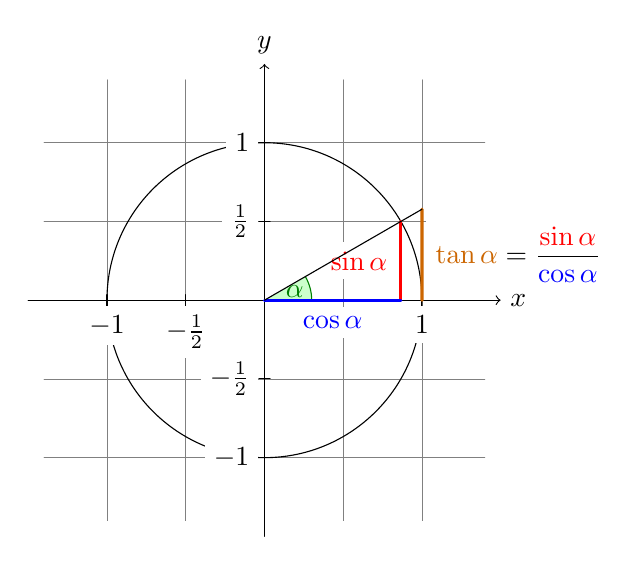
\begin{tikzpicture}[scale=2,cap=round]
    % Local definitions
    \def\costhirty{0.8660256}
  
    % Colors
    \colorlet{anglecolor}{green!50!black}
    \colorlet{sincolor}{red}
    \colorlet{tancolor}{orange!80!black}
    \colorlet{coscolor}{blue}
  
    % Styles
    \tikzstyle{axes}=[]
    \tikzstyle{important line}=[very thick]
    \tikzstyle{information text}=[rounded corners,fill=red!10,inner sep=1ex]
  
    % The graphic
    \draw[style=help lines,step=0.5cm] (-1.4,-1.4) grid (1.4,1.4);
  
    \draw (0,0) circle (1cm);
  
    \begin{scope}[style=axes]
      \draw[->] (-1.5,0) -- (1.5,0) node[right] {$x$};
      \draw[->] (0,-1.5) -- (0,1.5) node[above] {$y$};
  
      \foreach \x/\xtext in {-1, -.5/-\frac{1}{2}, 1}
        \draw[xshift=\x cm] (0pt,1pt) -- (0pt,-1pt) node[below,fill=white]
              {$\xtext$};
  
      \foreach \y/\ytext in {-1, -.5/-\frac{1}{2}, .5/\frac{1}{2}, 1}
        \draw[yshift=\y cm] (1pt,0pt) -- (-1pt,0pt) node[left,fill=white]
              {$\ytext$};
    \end{scope}
  
    \filldraw[fill=green!20,draw=anglecolor] (0,0) -- (3mm,0pt) arc(0:30:3mm);
    \draw (15:2mm) node[anglecolor] {$\alpha$};
  
    \draw[style=important line,sincolor]
      (30:1cm) -- node[left=1pt,fill=white] {$\sin \alpha$} +(0,-.5);
  
    \draw[style=important line,coscolor]
      (0,0) -- node[below=2pt,fill=white] {$\cos \alpha$} (\costhirty,0);
  
    \draw[style=important line,tancolor] (1,0) --
      node [right=1pt,fill=white]
      {
        $\displaystyle \tan \alpha \color{black}=
        \frac{{\color{sincolor}\sin \alpha}}{\color{coscolor}\cos \alpha}$
      } (intersection of 0,0--30:1cm and 1,0--1,1) coordinate (t);
  
    \draw (0,0) -- (t);
  
  \end{tikzpicture}
\end{frame}

\begin{frame}{3.2.2 手绘图}
  \tikzstyle{every picture}+=[remember picture]
  \[  y =  \tikz[baseline]{\node[fill=blue!50,anchor=base] (t1){$a$};} x +
  \tikz[baseline]{\node[fill=red!50,anchor=base ] (t2){$b$};}
  \]
  \begin{itemize}
  \item \tikz\node [fill=blue!50,draw,circle] (n1) {};\ 斜率
  \item \tikz\node [fill=red!50,draw,circle] (n2) {};\ 截距
  \end{itemize}
  \begin{tikzpicture}[overlay,>=latex]
  \path[blue,->] (n1.north) edge [out= 60, in= 135] (t1.north west);
  \path[red,->] (n2.south) edge [out=-70, in=-110] (t2.south);
  \end{tikzpicture}
\end{frame}

\section[公式]{公式的排版}

        \begin{frame}{2.3 公式}
            \begin{equation}
            \frac{\mathrm{d}\mathbf{\mathrm{x}}(t)}{\mathrm{d}t} = A\mathbf{\mathrm{x}}(t)+ B\mathbf{\mathrm{u}}(t)\text{。}
            \label{eq:control}
            \end{equation}
            
            其中:
            \begin{itemize}
            \item 向量$\mathbf{\mathrm{x}}(t)$表示$N$个在$t$时
            \item $A$表示$N$个度
            \item $\mathbf{\mathrm{u}}$
            \item $B$表示位点
            \end{itemize}
            
            %\pause
            \begin{alertblock}{注意}
            此公式用于...,不适用于.....。
            \end{alertblock}
        \end{frame}

\section[列表]{列表的排版}

        \begin{frame}{2.3 列表}
            \begin{table}
            \begin{tabular}{llc}
                First Name & Surname  & Year of Birth \\ \midrule
                Albert     & Einstein & 1879          \\
                Marie      & Curie    & 1867          \\
                Thomas     & Edison   & 1847          \\
            \end{tabular}
            \caption{The great minds of the 19th century}
            \end{table}
            废话一大堆
        \end{frame}

\section[代码]{代码高亮}

        \begin{frame}[fragile]
        \frametitle{2.4 代码高亮}
        C代码:
        \begin{minted}[mathescape,
                    linenos,     % displays the line numbers
                    frame=leftline,
                baselinestretch=0.5]{csharp}
        /*
        这里可以显示公式:
        $\pi=\lim_{n\to\infty}\frac{P_n}{d}$ where $P$ is the perimeter
        of an $n$-sided regular polygon circumscribing a
        circle of diameter $d$.
        */
        const double pi = 3.1415926535
        \end{minted}

        python代码:
        \begin{minted}[mathescape, linenos]{python}
        # Returns $\sum_{i=1}ˆ{n}i$
        # 多样注释格式和缩进,行码
        def sum_from_one_to(n):
            r = range(1, n + 1)
            return sum(r)
        \end{minted}
        \end{frame}

% \section{文献引用}
%         \begin{frame}
%         \frametitle{宇宙大爆炸的定义}
%         $x^2+y^2=z^2$\bcite{bcite1}
%         % \pause
%         \begin{definition}
%         \point{宇宙大爆炸}:$(X_0,Y_0)$当且仅当$\forall \epsilon >0$\bcite{bcite2}。
%         \end{definition}
%         \end{frame}

%----------------------------------------

\section[{动画} ]{左右分栏和图形动画} 

        \begin{frame}
            \begin{columns}[c] % The "c" option specifies centered vertical alignment while the "t" option is used for top vertical alignment
            \column{.45\textwidth} % Left column and width
            \begin{figure}
                \begin{center}
                \tikzstyle{linktype1visible}= [visible on=<{4-}>]
                \tikzstyle{linktype1previsible}= [visible on=<{1-3}>]
                \tikzstyle{nodetype1visible}= [visible on=<{4-}>]
                \tikzstyle{nodetype1previsible}= [visible on=<{1-3}>]
                \tikzstyle{linktype2visible}= [visible on=<{5-}>]
                \tikzstyle{scalestyle}= [scale=0.7]
                \begin{tikzpicture}
                \node[scalestyle, visible on=<{1,2,3,4}>, nodetype1pre] (N-1) at (0, 1) {1};
                \node[scalestyle, visible on=<{5-}>, nodetype1] (N-1) at (0, 1) {1};
                \foreach \name/\x in {2/2, 3/3, 4/4, 5/5}
                {
                \node[scalestyle, nodetype1pre, nodetype1previsible] (N-\name) at (0, \x) {$\name$};
                \node[scalestyle, nodetype1, nodetype1visible] (N-\name) at (0, \x) {$\name$};
                }
                \foreach \name/\x/\y in {6/1/4, 7/2/5, 8/3/4, 9/2/3}
                {
                \node[scalestyle, nodetype1pre, nodetype1previsible] (N-\name) at (\x, \y) {$\name$};
                \node[scalestyle, nodetype1, nodetype1visible] (N-\name) at (\x, \y) {$\name$};
                }
                \foreach \name/\x/\y in {10/-1/2, 11/-2/2}
                {
                \node[scalestyle, nodetype1pre, nodetype1previsible] (N-\name) at (\x, \y) {$\name$};
                \node[scalestyle, nodetype1, nodetype1visible] (N-\name) at (\x, \y) {$\name$};
                }
                \foreach \from/\to in {1/2, 2/3, 3/4, 4/5, 6/7, 7/8, 8/9, 9/6}
                {
                \draw[unlinktype1, linktype1previsible] (N-\from) -- (N-\to);
                }
                \draw[unlinktype1](N-4) -- (N-6);
                \draw[unlinktype1](N-2) -- (N-10);
                \path[unlinktype1] (N-5) edge [loop above] ();
                \draw[linktype1pre, linktype1previsible] (N-10) .. controls + (up:0.5cm) .. (N-11);
                \draw[linktype1pre, linktype1previsible] (N-11) .. controls + (down:0.5cm) .. (N-10);

                \foreach \from/\to in {1/2, 2/3, 3/4, 4/5, 6/7, 7/8, 8/9, 9/6}
                {
                \draw[linktype1, linktype1visible] (N-\from) -- (N-\to);
                }
                \draw[linktype1, linktype1visible] (N-10) .. controls + (up:0.5cm) .. (N-11);
                \draw[linktype1, linktype1visible] (N-11) .. controls + (down:0.5cm) .. (N-10);
                \draw[linktype2, linktype2visible] (0,-1) --  (0,0.7);
                \end{tikzpicture}
                \end{center}
            \end{figure}
            \column{.45\textwidth} % Left column and width
            \begin{itemize}
                    \item<1-| alert@1>
                第一条说明
                    \item<4-| alert@4>
                第二条说明
                    \item<5-| alert@5>
                第三条说明
                    \item<8-| alert@8>
                第四条说明
            \end{itemize}
            \visible<2>{\fadetitle{这是一个透明标题}}
            \end{columns}
            \visible<6>{
            \fadetitle{\(\displaystyle
            A=\left( 
                \begin{array}{*{20}{rcccccccccl}}
                0&0&0&0&0&0&0&0&0&0&0\\
                a&0&0&0&0&0&0&0&0&0&0\\
                0&b&0&0&0&0&0&0&0&c&0\\
                \end{array}
            \right)
            \)
            }
        }
        \end{frame}
%------------------------------------------------

\begin{frame}
    \begin{figure}
        \begin{center}
            \tikzstyle{nodetype1visible}= [visible on=<{2-}>]
            \tikzstyle{nodetype1previsible}= [visible on=<{1}>]
            \tikzstyle{linktype2visible}= [visible on=<{3-}>]
            \tikzstyle{linktype1visible}= [visible on=<{2-}>]
            \tikzstyle{linktype1previsible}= [visible on=<{1}>]

            \begin{minipage}[b]{0.45\linewidth}
            \begin{tikzpicture}[scale=0.7]
            %-------------------------------------
            \node[unnodetype1,label=below left:$x_2$] (x2)  at (0,0) {};
            \node[unnodetype1,label=above right:$x_1$] (x1)  at (2,1) {};
            \node[nodetype1pre,nodetype1previsible,label=below right:$x_4$] (x4)  at (2,-1) {};
            \node[nodetype1,nodetype1visible,label=below right:$x_4$] (x4)  at (2,-1) {};
            \node[unnodetype1,label=below right:$x_3$] (x3)  at (4,0) {};
            %-------------------------------------
            \draw[-latex] (x1) -- (x2);
            \draw[-latex] (x1) -- (x3);
            \draw[linktype1pre,linktype1previsible] (x1) -- (x4);
            \draw[linktype1,linktype1visible] (x1) -- (x4);
            \draw[linktype2,linktype2visible] (2,3) node [right] {$u_1$} --  (x1);
            \draw[linktype2,linktype2visible] (4,2) node [right] {$u_3$}-- (x3);
            \draw[linktype2,linktype2visible] (0,2) node [left] {$u_2$}-- (x2);
            %-------------------------------------
            \end{tikzpicture}
            \end{minipage}
            \quad
            \pause
            \begin{minipage}[b]{0.45\linewidth}
            \begin{tikzpicture}[scale=0.7]
            %-------------------------------------
            \node[nodetype1pre,nodetype1previsible,label=below left:$x_2$] (x2)  at (0,0) {};
            \node[nodetype1,nodetype1visible,label=below left:$x_2$] (x2)  at (0,0) {};
            \node[unnodetype1,label=above right:$x_1$] (x1)  at (2,1) {};
            \node[unnodetype1,label=below left:$x_4$] (x4)  at (2,-1) {};
            \node[unnodetype1,label=below right:$x_3$] (x3)  at (4,0) {};
            %-------------------------------------
            \draw[-latex] (x1) -- (x4);
            \draw[-latex] (x1) -- (x3);
            \draw[linktype1pre,linktype1previsible] (x1) -- (x2);
            \draw[linktype1,linktype1visible] (x1) -- (x2);
            \draw[linktype2, linktype2visible] (2,3) node [right] {$u_1$} --  (x1);
            \draw[linktype2, linktype2visible] (4,2) node [right] {$u_3$}-- (x3);
            \draw[linktype2, linktype2visible] (4,-2) node [right] {$u_4$}-- (x4);
            %-------------------------------------
            \end{tikzpicture}
            \end{minipage}
            \begin{minipage}[b]{0.45\linewidth}
            \begin{tikzpicture}[scale=0.7]
            %-------------------------------------
            \node[unnodetype1,label=below left:$x_2$] (x2)  at (0,0) {};
            \node[unnodetype1,label=above right:$x_1$] (x1)  at (2,1) {};
            \node[unnodetype1,label=below left:$x_4$] (x4)  at (2,-1) {};
            \node[nodetype1pre,nodetype1previsible,label=below right:$x_3$] (x3)  at (4,0) {};
            \node[nodetype1,nodetype1visible,label=below right:$x_3$] (x3)  at (4,0) {};
            %-------------------------------------
            \draw[-latex] (x1) -- (x2);
            \draw[-latex] (x1) -- (x4);
            \draw[linktype1pre, linktype1previsible] (x1) -- (x3);
            \draw[linktype1, linktype1visible] (x1) -- (x3);
            \draw[linktype2,linktype2visible] (2,3) node [right] {$u_1$} --  (x1);
            \draw[linktype2,linktype2visible] (4,-2) node [right] {$u_4$}-- (x4);
            \draw[linktype2,linktype2visible] (0,2) node [left] {$u_2$}-- (x2);
            %-------------------------------------
            \node[unnodetype1,label=right:Original node] at (6.25,2) {};
            \visible<2->{\node[nodetype1,nodetype1visible,label=right:Matched node] at (6.25,1) {};}
            \draw[linktype1,linktype1visible] (5, 0) -- (6.5, 0) node [right] {Link type 1};
            \draw[linktype2,line after snake=2mm, linktype2visible] (5,-1) --(6.5,-1) node [right] {Link type 2};
            \end{tikzpicture}
            \end{minipage}
        \end{center}
    \end{figure}
\end{frame}

%------------------------------------------------

\section[思维导图]{思维导图} 
    \begin{frame}
    \frametitle{思维导图}
    \setbeamercovered{invisible}
        \begin{tikzpicture}[scale=0.6, transform shape]
        \bf
        \centering
        \path[mindmap,concept color=structure.fg,text=white]
            node[concept] {Beamer模板}
            [clockwise from=0]
            child[concept color=green!30!black, visible on=<{2-}>] {
            node[concept] {tikz作图}
            [clockwise from=90]
            child { node[concept] {节点} }
            child { node[concept] {边} }
            child { node[concept] {样式定义} }
            child { node[concept] {样式分配} }
            }
            child[concept color=blue!80!black, visible on=<{3-}>] {
            node[concept] {代码高亮}
            [clockwise from=-30]
            child { node[concept] {支持所有代码} }
            child { node[concept] {支持公式} }
            }
            child[concept color=red!70!structure.fg, visible on=<{4-}>] { 
            node[concept] {文献} 
            [clockwise from=-30]
            child { node[concept] {格式多样} }
            child { node[concept] {引用方便} }
            }
            child[concept color=orange!70!structure.fg, visible on=<{5-}>] { 
            node[concept] {主题} 
            [clockwise from=-90]
            child { node[concept] {主题颜色} }
            child { node[concept] {背景和前景} }
            child { node[concept] {字体} }
            child { node[concept] {图形} }
            };
        \end{tikzpicture}
        \visible<6->{\fadetitle{\Huge{\centerline{谢谢}}}}
    \end{frame}


        % \begin{frame}[noframenumbering,allowframebreaks, plain]
        %     \frametitle<presentation>{References}
        %     \printbibliography
        % \end{frame}        

\end{document} 